% !TEX program = xelatex
% =====================================================================
% Strategie et sources -- notes pour la defense / validation
% Probleme 1, GEI723 (Automne 2026) : locomotion hexapode
% Compilation : xelatex strategie ; bibtex strategie ; xelatex strategie ; xelatex strategie
% =====================================================================
\documentclass[11pt]{article}
\usepackage[letterpaper, margin=2.2cm]{geometry}
\usepackage{fontspec}
\usepackage{polyglossia}
\setdefaultlanguage{french}
\usepackage{xcolor}
\usepackage{graphicx}
\usepackage{booktabs}
\usepackage{tabularx}
\usepackage{array}
\usepackage{amsmath}
\usepackage{enumitem}
\usepackage[hidelinks]{hyperref}
\usepackage{titlesec}

% ---------------------------------------------------------------- polices (memes que l'affiche)
\setmainfont{IBMPlexSans}[Path=fonts/, Extension=.ttf, UprightFont=*-Regular,
  BoldFont=*-SemiBold, ItalicFont=*-Italic]
\setmonofont{IBMPlexMono}[Path=fonts/, Extension=.ttf, UprightFont=*-Regular,
  BoldFont=*-SemiBold, Scale=0.92]
\newfontfamily\condensed{IBMPlexSansCondensed}[Path=fonts/, Extension=.ttf,
  UprightFont=*-Bold, BoldFont=*-Bold]

\definecolor{encre}{HTML}{16161A}
\definecolor{gris}{HTML}{4A4A52}
\definecolor{bleu}{HTML}{2A78D6}
\definecolor{orange}{HTML}{EB6834}
\definecolor{fondbloc}{HTML}{F4F2EC}
\definecolor{alerte}{HTML}{C2410C}

\titleformat{\section}{\condensed\Large\color{encre}}{\color{bleu}\thesection}{0.6em}{}
\titleformat{\subsection}{\bfseries\large}{\thesubsection}{0.5em}{}
\titlespacing*{\section}{0pt}{1.6em}{0.6em}
\setlength{\parindent}{0pt}
\setlength{\parskip}{0.55em}
\setlist{itemsep=0.25em, topsep=0.3em}
\renewcommand{\arraystretch}{1.3}

% Une etape de la demarche : question, idee, source, ce qu'on a fait
\newcommand{\champ}[2]{\par\noindent\textbf{\color{bleu}#1} #2\par}
% Encadre de mise en garde
\newcommand{\attention}[2]{\par\noindent\colorbox{fondbloc}{\parbox{\dimexpr\linewidth-2\fboxsep}{%
  \textbf{\color{alerte}#1}\quad #2}}\par}
\newcommand{\code}[1]{\texttt{#1}}

\begin{document}

{\condensed\fontsize{24pt}{28pt}\selectfont Stratégie et sources\par}
\vspace{0.3em}
{\large Problème 1 --- Locomotion hexapode par un réseau de neurones à décharges\par}
\vspace{0.2em}
{\color{gris} GEI723 · Automne 2026 · Raphaël Barrette, Émile [NOM] · Notes pour la défense\par}
\vspace{0.8em}
\hrule
\vspace{0.6em}

Ce document présente notre démarche sur papier, dans l'ordre où les problèmes se posent. Chaque étape
suit le même format : \textbf{la question}, \textbf{l'idée retenue}, \textbf{la source} (citée
précisément) et \textbf{ce que nous avons fait} dans le réseau.

% ====================================================================
\section{Deux points à ne pas confondre}

\attention{Un tripode n'est pas un côté.}{Les trois pattes d'un même côté ne se lèvent jamais
ensemble (le corps basculerait). Un tripode mélange les deux côtés : \textbf{G1, D2, G3} contre
\textbf{D1, G2, D3}. Les pattes au sol forment toujours un triangle d'appui, deux d'un côté, une de
l'autre.}

\vspace{0.4em}
\attention{A et B ne s'auto-inhibent pas.}{Ils s'inhibent \emph{mutuellement} (chacun freine
l'autre, poids W\_AB). Ce qui freine un neurone \emph{lui-même}, c'est sa fatigue, l'adaptation $a$.}

% ====================================================================
\section{La démarche, étape par étape}

% --------------------------------------------------------------------
\subsection*{Étape 1 --- Comment faire avancer six pattes sans tomber ?}

\champ{Solution naïve écartée.}{Lever et avancer les trois pattes d'un même côté, puis celles de
l'autre côté. Aucune patte ne soutient alors le côté levé : le corps bascule.}
\champ{Idée retenue.}{La \textbf{démarche tripode} : deux groupes de trois pattes alternent. Pendant
qu'un tripode se lève et avance, l'autre est au sol et pousse ; trois pattes forment toujours un
triangle d'appui.}
\champ{Source.}{Otis (2004), fig.~5.2(a), p.~110 \cite{otis2004} : la figure montre un damier
qui correspond exactement à notre règle.}
\champ{Ce que nous avons fait.}{Chaque patte $(k, s)$ ($k$ = segment, $s$ = 0 gauche / 1 droite)
reçoit le groupe
\[ \text{groupe}(k, s) = (k + s) \bmod 2 . \]
Pour $N = 3$ paires, on obtient G1, D2, G3 (groupe 0) et D1, G2, D3 (groupe 1). La même règle
fonctionne pour n'importe quel nombre de paires, ce qui permet de passer à 200 paires en changeant
une seule variable.}

% --------------------------------------------------------------------
\subsection*{Étape 2 --- Comment produire un rythme régulier qui fait alterner les tripodes ?}

\champ{Idée retenue.}{Deux neurones, A et B, qui \textbf{s'inhibent mutuellement} : quand l'un
décharge, l'autre est bloqué. A commande la phase 1, B la phase 2. C'est le générateur central de
rythme (CPG).}
\champ{Source.}{Otis (2004), fig.~5.1, p.~108 \cite{otis2004} : deux neurones en inhibition
mutuelle ; p.~107 : « la fatigue d'un neurone permet à l'autre de s'activer ». Le fait qu'une
seule entrée règle la vitesse vient de Beer et al. (1992), p.~358 \cite{beer1992}.}
\champ{Ce que nous avons fait (notre réglage).}{}
\begin{itemize}
  \item \textbf{Adaptation forte} : à chaque décharge, $a$ augmente de 1,5. La cible du voltage
        $v_\infty = I - a - g_i$ passe sous le seuil, donc le neurone ne peut pas décharger deux
        fois de suite : \textbf{une seule décharge par phase}.
  \item \textbf{Récupération} ($\tau_a$ = 200~ms) : elle fixe la durée du cycle, environ 197~ms
        à I\_drive = 2.
  \item \textbf{Inhibition mutuelle} (W\_AB = 4) : elle empêche A et B de décharger trop près
        l'un de l'autre et les garde en \textbf{antiphase}.
  \item \textbf{Vitesse} : I\_drive est la seule commande de vitesse. Plus il est grand, moins le
        neurone doit récupérer avant de redécharger, donc plus le cycle est court
        (3,4~Hz à I\_drive = 1,5 ; 7,6~Hz à 3).
\end{itemize}

\begin{center}
  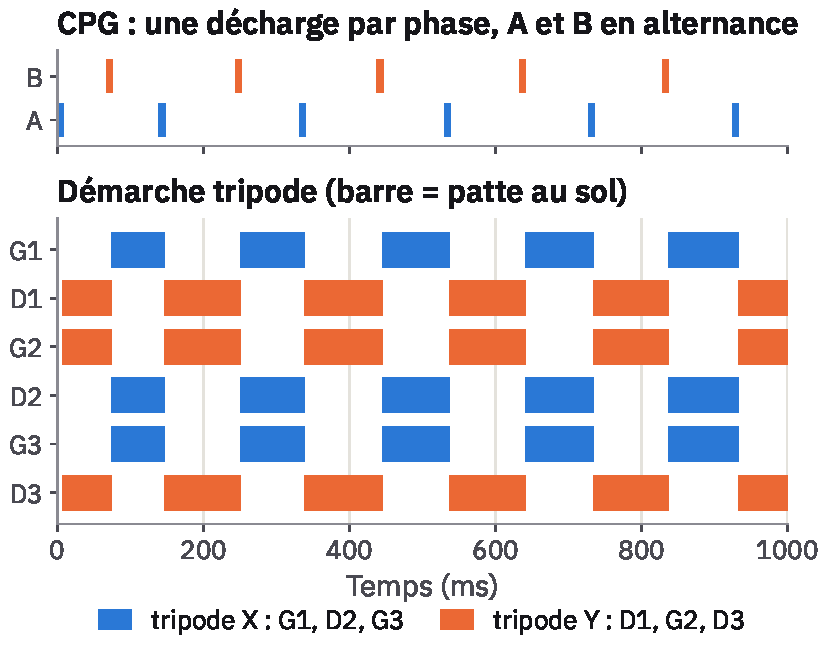
\includegraphics[width=0.78\linewidth]{figures/p1_cpg_demarche}\\[0.3em]
  {\small\color{gris} A et B alternent ; chaque décharge fait changer de rôle les deux tripodes.}
\end{center}

% --------------------------------------------------------------------
\subsection*{Étape 3 --- Quelles commandes envoyer à chaque patte ?}

\champ{Idée retenue.}{Le minimum pour décrire un pas : quatre motoneurones par patte,
\textbf{LEVER, POSER, AVANT, ARRIÈRE}. Une décharge signifie « exécute cette commande
maintenant ».}
\champ{Source.}{Beer et al. (1992), fig.~2, p.~359 \cite{beer1992} : leur patte a trois
motoneurones (pied, avant, arrière). Nous avons séparé « pied » en LEVER et POSER.}
\champ{Ce que nous avons fait.}{}
\begin{itemize}
  \item Le neurone du CPG qui donne le \emph{swing} à une patte excite son LEVER ; l'autre excite
        son POSER. Le poids W\_MOT = 1,5 dépasse le seuil (1) : une décharge suffit.
  \item LEVER $\dashv\vdash$ POSER et AVANT $\dashv\vdash$ ARRIÈRE s'inhibent (W\_CONTRA = 3) : jamais deux commandes
        contradictoires en même temps.
  \item \textbf{Remarque :} pour la marche avant \emph{seulement}, on pourrait brancher
        swing → AVANT et stance → ARRIÈRE directement, et cela fonctionnerait. Le problème
        apparaît à l'étape suivante.
\end{itemize}

% --------------------------------------------------------------------
\subsection*{Étape 4 --- Comment changer de direction sans recâbler ? (contribution originale)}

\champ{Problème.}{En marche arrière, il faut l'inverse : swing → ARRIÈRE et stance → AVANT.
AVANT doit donc décharger dans deux cas :
\[ \text{AVANT} = (\text{swing} \wedge \text{mode avant}) \vee (\text{stance} \wedge \text{mode arrière}) . \]
C'est un \textbf{XNOR} entre la phase et le mode.}

\champ{Pourquoi un seul neurone ne suffit pas.}{Supposons qu'AVANT reçoive le swing (poids
$w_{sw}$), le stance ($w_{st}$) et un biais $b$ qui dépend du mode. Il faudrait :}

\begin{center}
\begin{tabular}{lll}
  \toprule
  \textbf{Mode} & \textbf{Swing → AVANT} & \textbf{Stance → AVANT}\\ \midrule
  avant   & $w_{sw} + b_{av} > 1$ (décharge) & $w_{st} + b_{av} < 1$ (silence)\\
  arrière & $w_{sw} + b_{ar} < 1$ (silence)  & $w_{st} + b_{ar} > 1$ (décharge)\\ \bottomrule
\end{tabular}
\end{center}

La colonne swing impose $b_{av} > b_{ar}$ ; la colonne stance impose $b_{ar} > b_{av}$ :
\textbf{contradiction}. Le XNOR n'est pas linéairement séparable ; il faut une couche cachée.

\champ{Solution : quatre interneurones « ET » par patte.}{Chacun répond à une question :}

\begin{center}
\begin{tabularx}{0.92\linewidth}{>{\ttfamily}l X l}
  \toprule
  \textrm{\textbf{Interneurone}} & \textbf{Question} & \textbf{Si oui, il excite}\\ \midrule
  IN\_sw\_av & « La patte est levée : est-ce que je l'avance ? »   & AVANT\\
  IN\_sw\_ar & « La patte est levée : est-ce que je la recule ? »  & ARRIÈRE\\
  IN\_st\_av & « La patte est au sol : est-ce que je l'avance ? »  & AVANT\\
  IN\_st\_ar & « La patte est au sol : est-ce que je la recule ? » & ARRIÈRE\\ \bottomrule
\end{tabularx}
\end{center}

\champ{Comment le mode choisit la réponse.}{Seuls les IN dont la réponse est « oui » dans le mode
actuel reçoivent un \textbf{biais constant} B\_ET = 0,6. Ce biais est sous le seuil (0,6 < 1) :
à lui seul, il ne fait rien décharger. Le neurone du CPG est branché sur les mêmes IN que sur
LEVER (swing) ou POSER (stance) de la patte, avec un poids \textbf{W\_ET = 0,6}, lui aussi sous le
seuil. Il faut \textbf{les deux en même temps} : $0{,}6 + 0{,}6 = 1{,}2 > 1$.}

\champ{Source.}{Aucune : cette pièce est de nous.}

% --------------------------------------------------------------------
\subsection*{Étape 5 --- Ce qui se passe en marche avant}

\textbf{Avant la simulation}, le mode avant met le biais sur \code{IN\_sw\_av} et
\code{IN\_st\_ar} de toutes les pattes : ces IN attendent à $v = 0{,}6$. Les deux autres restent à
$v = 0$.

\textbf{Quand A décharge} (la commande arrive aux pattes 3~ms plus tard) :

\begin{center}
\small
\begin{tabularx}{\linewidth}{l X X}
  \toprule
  & \textbf{\color{bleu}Tripode X (G1, D2, G3)} : A lui donne le swing
  & \textbf{\color{orange}Tripode Y (D1, G2, D3)} : A lui donne le stance\\ \midrule
  Direct        & LEVER : $0 + 1{,}5 > 1$ → \textbf{décharge} & POSER : $0 + 1{,}5 > 1$ → \textbf{décharge}\\
  IN avec biais & IN\_sw\_av : $0{,}6 + 0{,}6 = 1{,}2 > 1$ → \textbf{décharge} & IN\_st\_ar : $0{,}6 + 0{,}6 = 1{,}2 > 1$ → \textbf{décharge}\\
  IN sans biais & IN\_sw\_ar : $0 + 0{,}6 < 1$ → rien & IN\_st\_av : $0 + 0{,}6 < 1$ → rien\\
  0,1~ms après  & IN\_sw\_av → \textbf{AVANT} & IN\_st\_ar → \textbf{ARRIÈRE}\\ \midrule
  Résultat      & \textbf{LEVER + AVANT} : la patte se lève et va vers l'avant
                & \textbf{POSER + ARRIÈRE} : la patte se pose et pousse ; le corps avance\\ \bottomrule
\end{tabularx}
\end{center}

\textbf{Ensuite}, A est fatiguée ($a$ + 1,5) et ne peut plus décharger. B, qui a récupéré de sa
propre décharge, décharge environ 100~ms plus tard : les deux tripodes échangent leurs rôles, et
ainsi de suite.

\textbf{Pour passer en marche arrière}, il suffit de déplacer le biais vers \code{IN\_sw\_ar} et
\code{IN\_st\_av}. Le CPG et toutes les connexions restent identiques.

% ====================================================================
\section*{Récapitulatif des sources}

\begin{center}
\small
\begin{tabularx}{\linewidth}{l X l}
  \toprule
  \textbf{Pièce du réseau} & \textbf{Ce qu'on y a pris} & \textbf{Source}\\ \midrule
  Tripode et règle $(k + s) \bmod 2$ & alternance de deux groupes de trois pattes & Otis, fig.~5.2(a), p.~110\\
  CPG à deux neurones & inhibition mutuelle ; la fatigue fait alterner & Otis, fig.~5.1, p.~107--108\\
  Vitesse & une seule entrée règle la fréquence & Beer et al., p.~358\\
  Motoneurones de patte & pied / avant / arrière ; pied séparé en LEVER / POSER & Beer et al., fig.~2, p.~359\\
  Interneurones « ET » & --- & original\\
  Compteur de virage & idée : raccourcir les pas d'un côté pour tourner & Otis, p.~112 (mécanisme original)\\ \bottomrule
\end{tabularx}
\end{center}

\attention{Pour la défense.}{L'énoncé valorise la démarche. Si la solution « un côté à la fois »
n'a pas été votre premier essai réel, présentez-la comme une option écartée (« la solution naïve
serait… ; elle échoue parce que… ») : c'est aussi convaincant, et c'est exact.}

\bibliographystyle{unsrt}
\bibliography{references}

\end{document}
